\HC[All]{Maybe one section of each of these}

\subsection{Prototype evaluation}

\begin{itemize}
%\item description of synthetic benchmarks
\item experimental setup
\item results and comments
\end{itemize}
This section evaluates the performance of Madeus with empty transitions.
Madeus is a model that relies on the description of an \emph{internal-net} (life-cycle) for each software component of that will be deployed. It is a low-level model, therefore the developer is responsible for the choices of actions performed in the transitions.

The aim is to evaluate Madeus independently of any specific transitions which is why these experiments are called \emph{dry-runs}. It means the transitions do not contain any action which allows to measure the overhead caused by Madeus.

% figures to add for assemblies
%Sequential

\begin{figure}[h]
  \begin{center}
    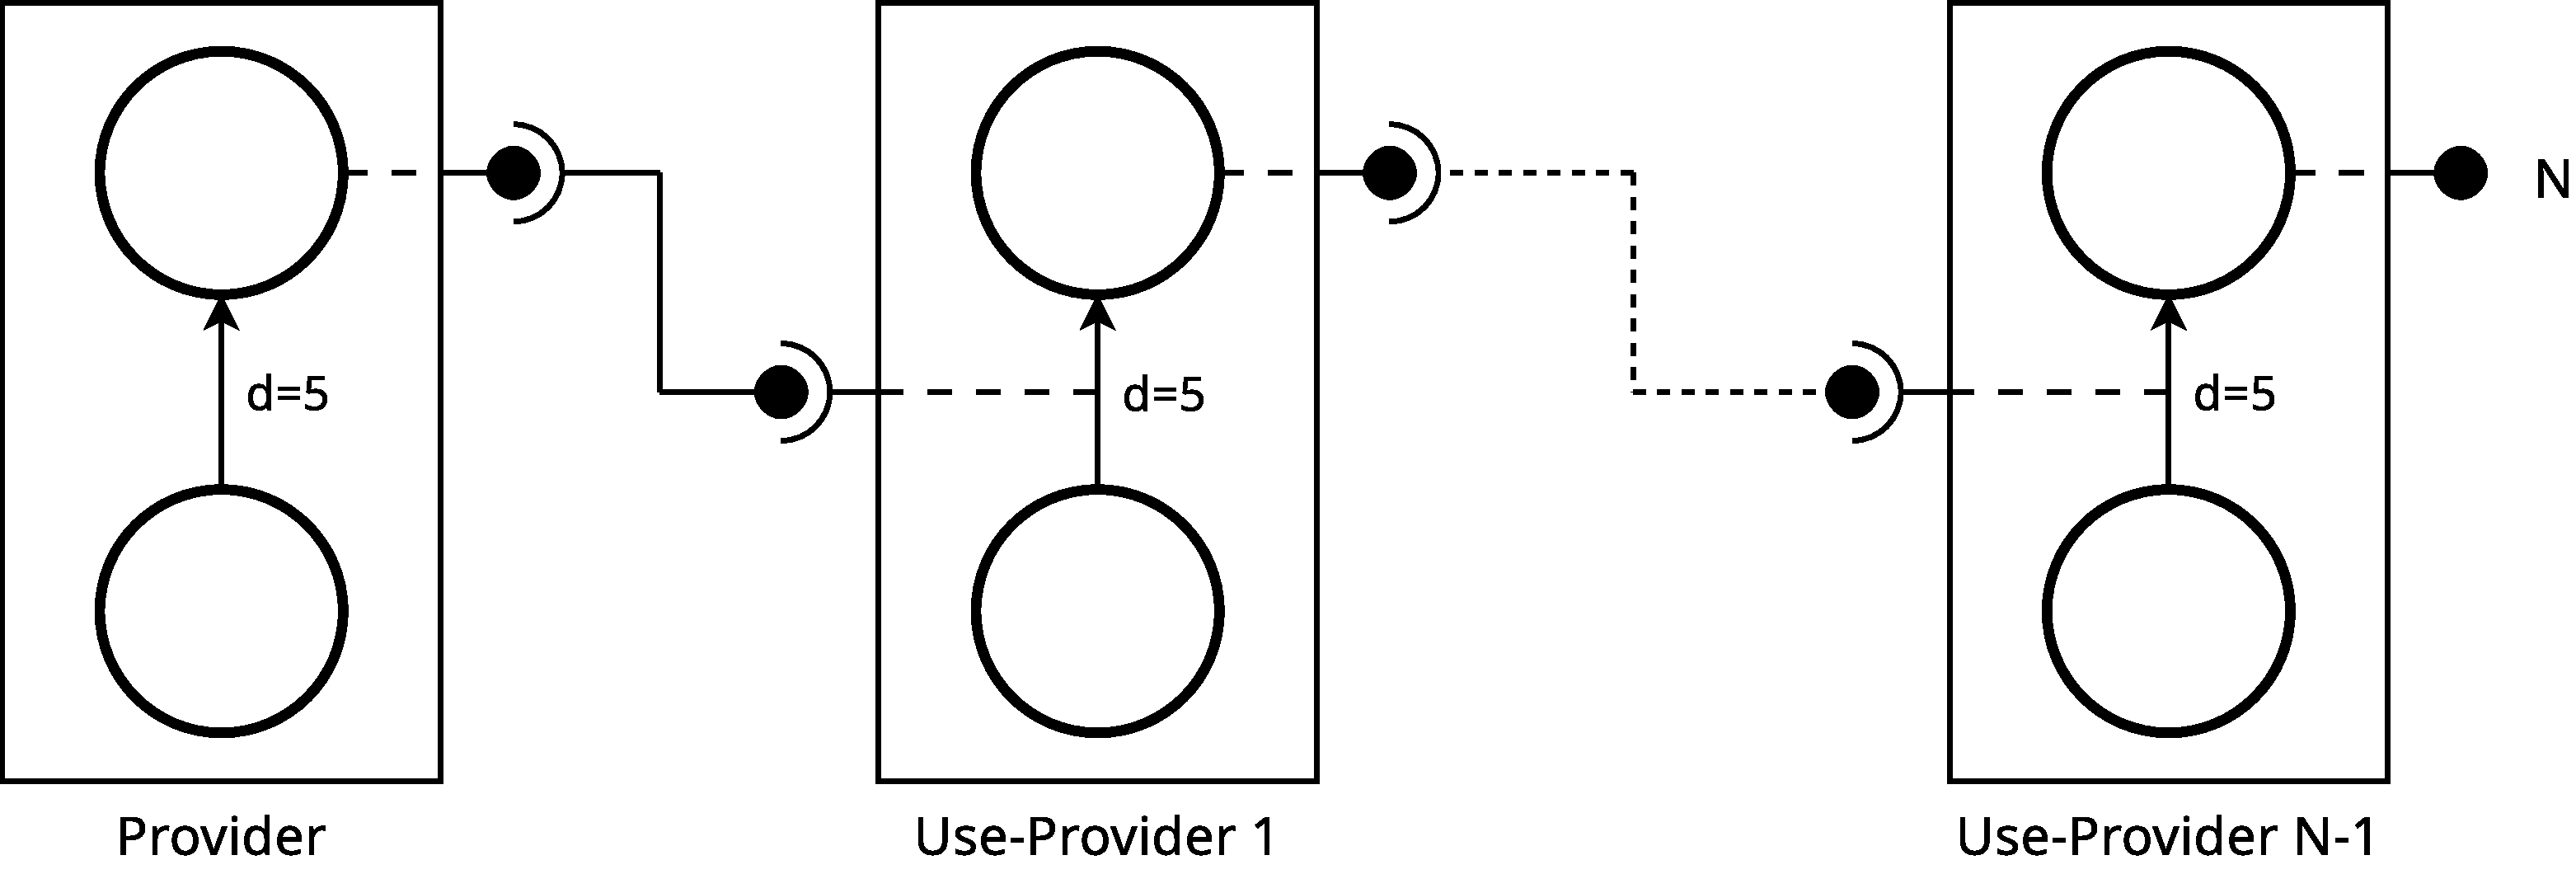
\includegraphics[width=0.4\textwidth]{./images/seq.pdf}
    \caption{The sequential assembly for the Madeus benchmark, with N components.}
    \label{fig:seq}
  \end{center}
\end{figure}

Three benchmarks compose this evaluation. The first benchmark is made with a sequential assembly written in Madeus, depicted in Figure~\ref{fig:seq}
and made of a chain of components: one \emph{provider} component made of a transition and two places, the final one providing a service, and \emph{N user-provider} components that are also composed of a transition and two places, but where the transition uses the provide port of the preceeding component. The components are connected and this results in a sequential execution.

A dry-run version of this assembly is built containing transitions that do nothing besides wait for a fixed amount of time. As it is a sequential assembly, the execution time should be increasing with the number of \emph{N} components.

\begin{figure}[h]
  \begin{center}
    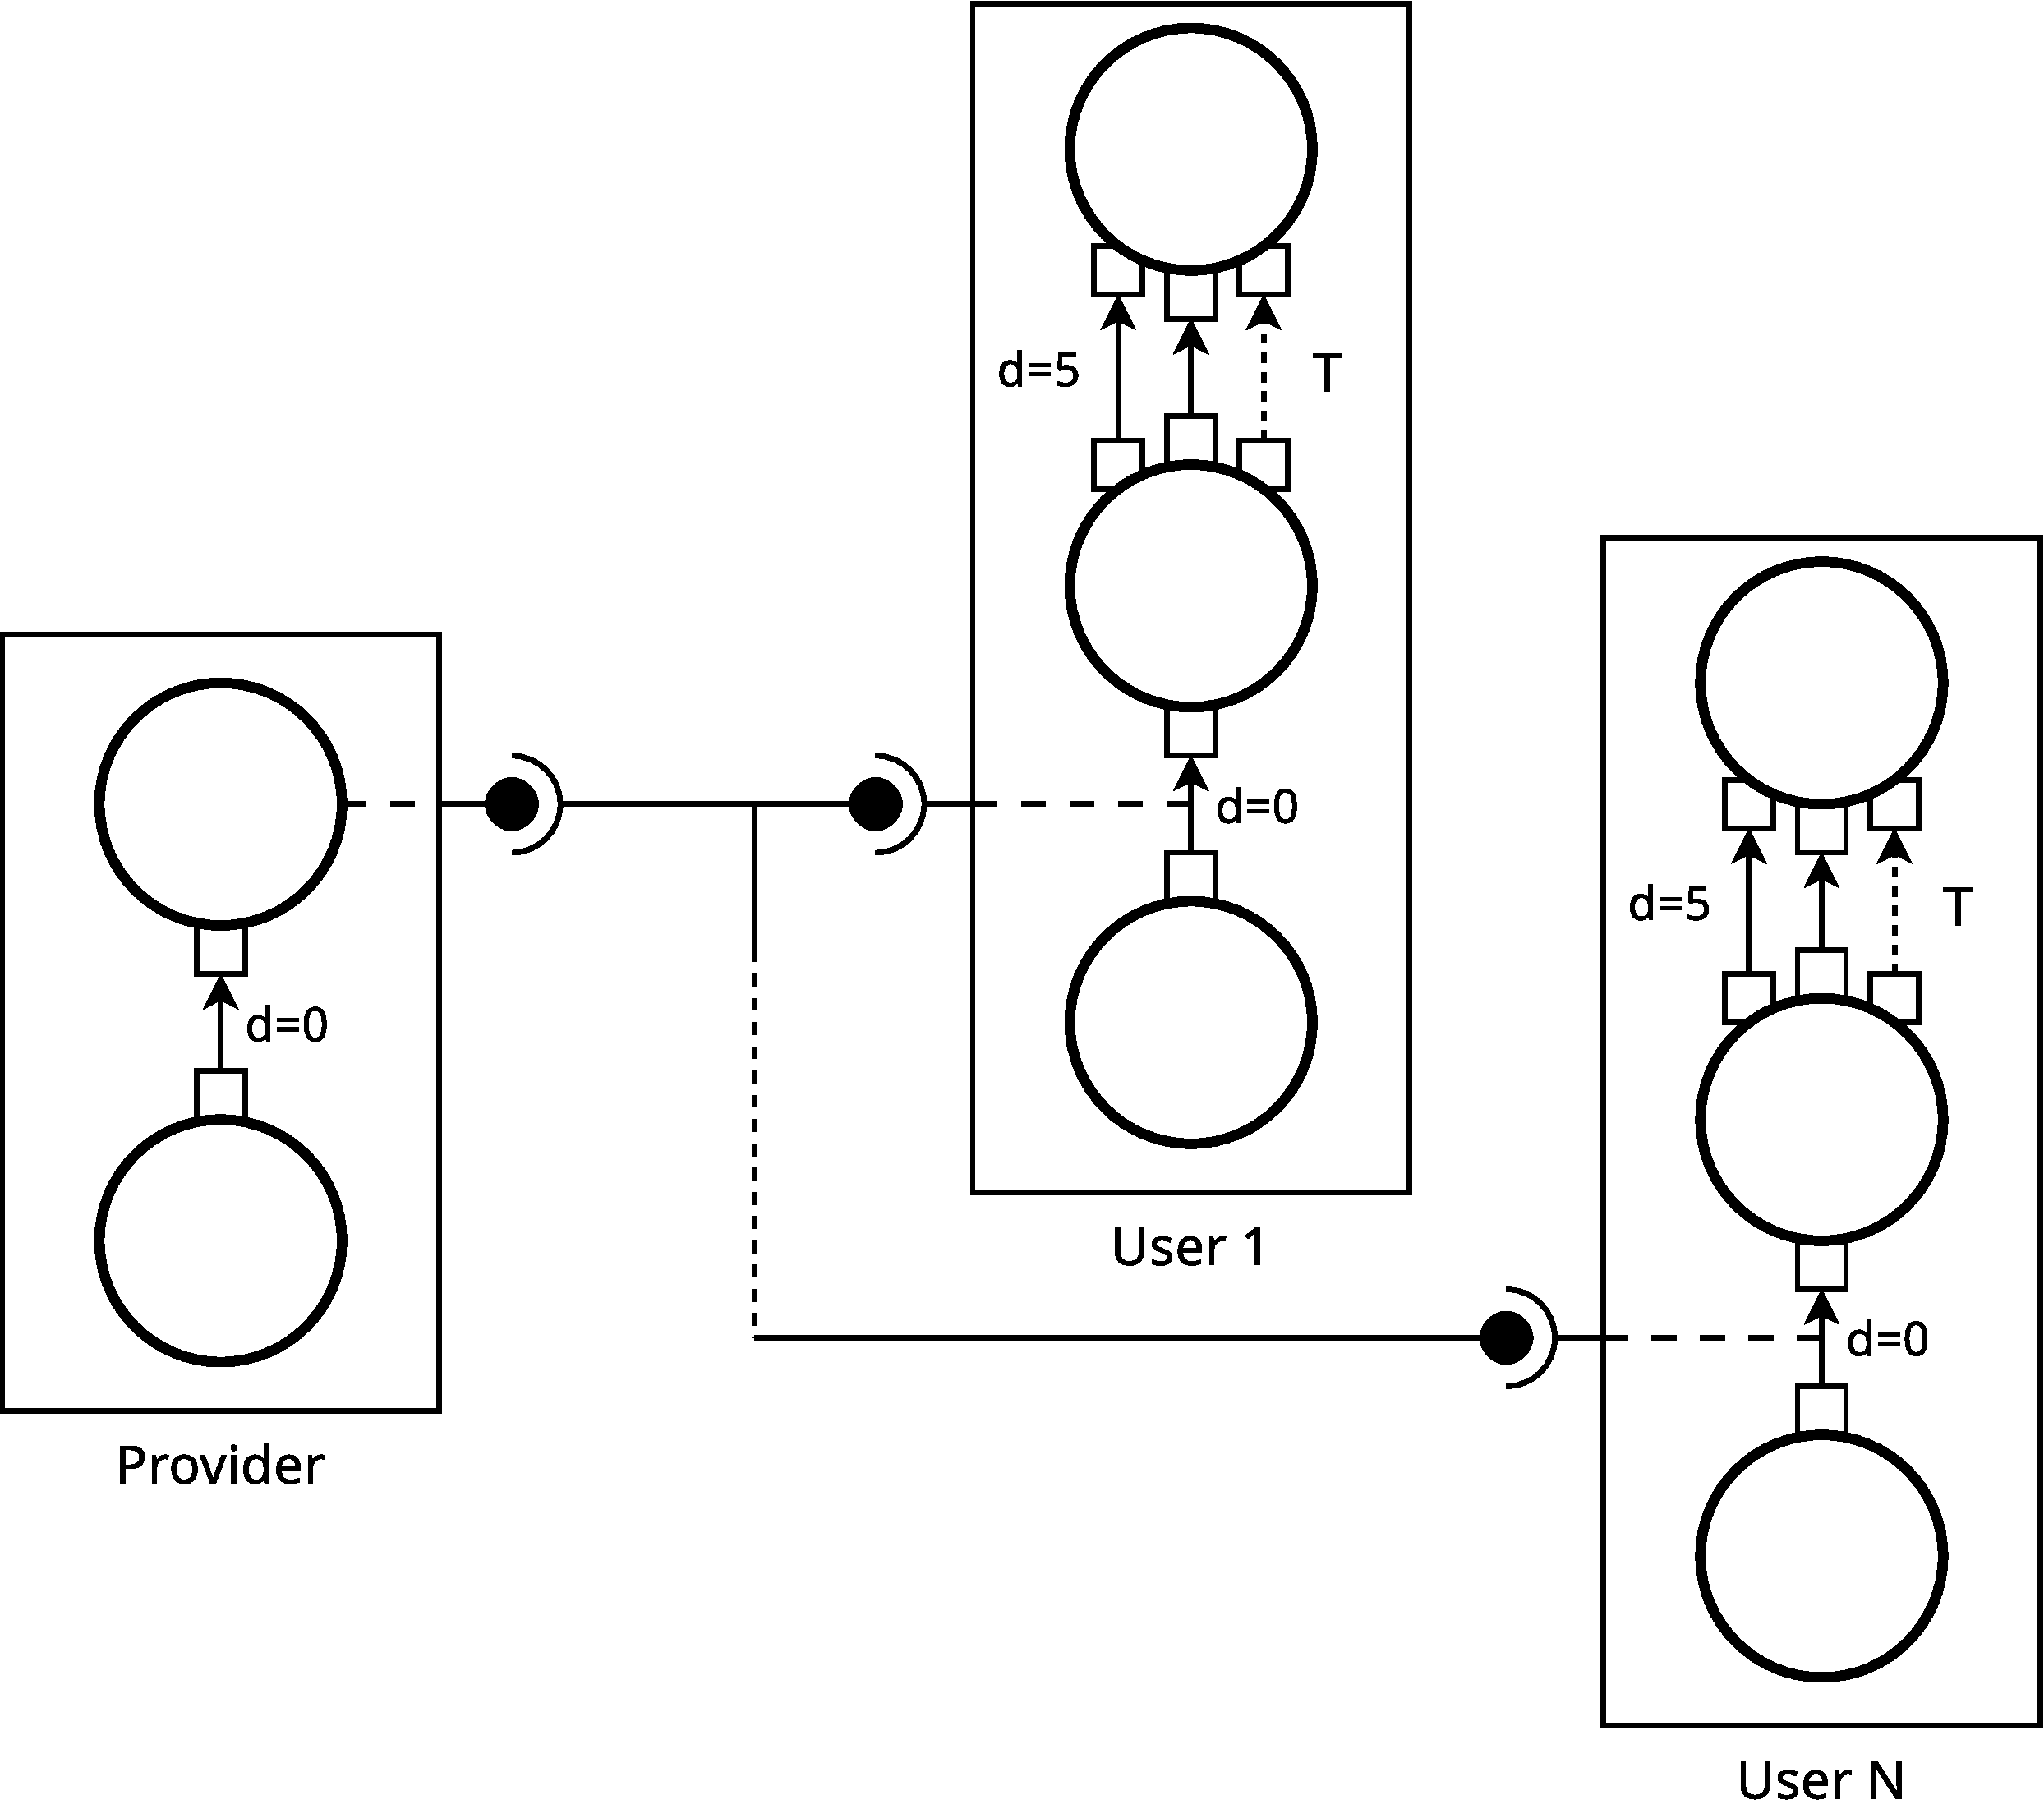
\includegraphics[width=0.4\textwidth]{./images/par.pdf}
    \caption{The parallel assembly for the Madeus benchmark, with N parallel components, and T parallel transitions.}
    \label{fig:par}
  \end{center}
\end{figure}

The second version of this assembly features a transition that calls an ssh connection and waits for a fixed amount of time, similar as for the dry-run version, before finishing. 

Two other benchmarks made with parallel assemblies written in Madeus, as depicted in Figure~\ref{fig:par}.
Their aim is to illustrate the performances of Madeus regardless of the components and the content of their transitions.

The first assembly evaluates the parallelism at the component level, when components are deployed simultaneously and the second one evaluates the parallelism at the transition level, when transitions are performed simultaneously.
The second and third benchmarks are made to evaluate the performances with parallelism both at the component level and at the transition level.

They use the same assembly that is composed of an initial \emph{provider} component and \emph{N parallel components} connected to the provider. Each component contains a first transition that uses the service provided by the provider component and \emph{T parallel transitions}. For the benchmark about component level parallelism, the number of components varies from 1 to 40 components and a fixed transition, while for the benchmark about transition level parallelism, the number of transitions varies from 1 to 20 %link to pictures

Each benchmark was run for ten iterations with a sleep time value of 5 seconds to have a coherent scale of results. They are both evaluated in \emph{dryrun} mode without any ssh connections and with \emph{ssh connections} active in the assembly between components, so as to allow visualisation of the eventual overhead of having these ssh connections.

\begin{figure}[h]
  \begin{center} 
    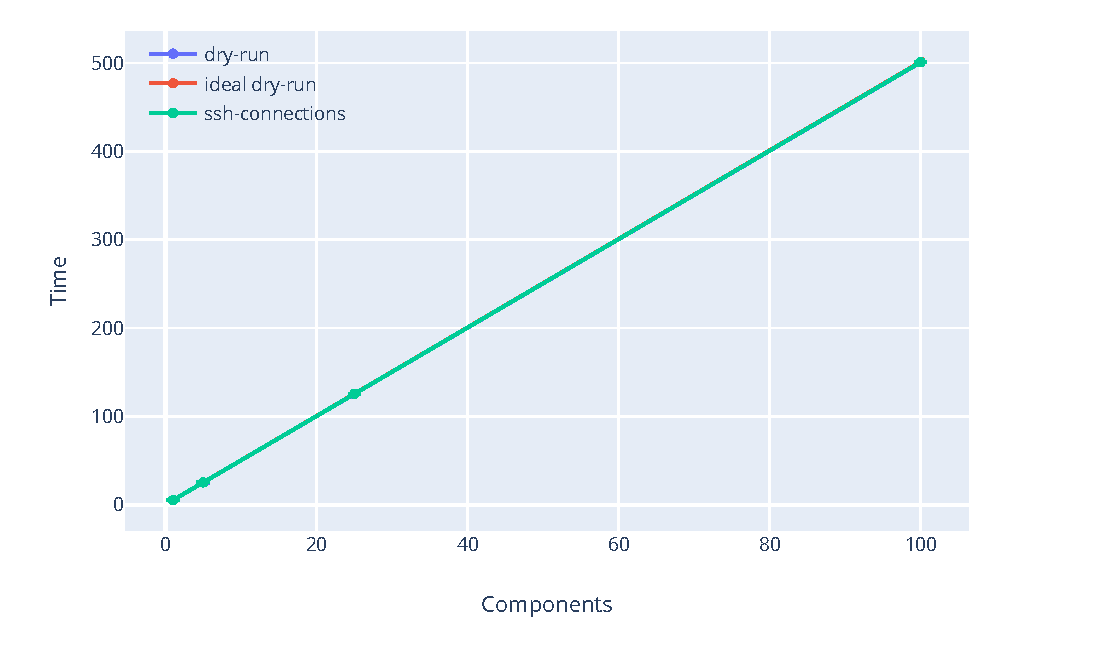
\includegraphics[width=0.5\textwidth]{./images/evaluations_sequential.pdf}
    \caption{Results of the sequential benchmark.}
    \label{fig:seqres}
  \end{center}
\end{figure}

For the sequential benchmark, we calculated the ideal curve as the sum of all sleep times added, since they are executed sequentially from the component assembly. The results show a linear increase in time and the \emph{dryrun} curve follows the \emph{ideal} curve closely, as can be seen on Figure~\ref{fig:seqres}. The difference between the \emph{ssh-connections} curve is hard to visualise but is slightly higher than the \emph{ideal} and \emph{dryrun} curves, a logical result as the number of ssh connections grows with each component added, but there is always only one ssh connection at the same time.

\begin{figure}[h]
  \begin{center} 
    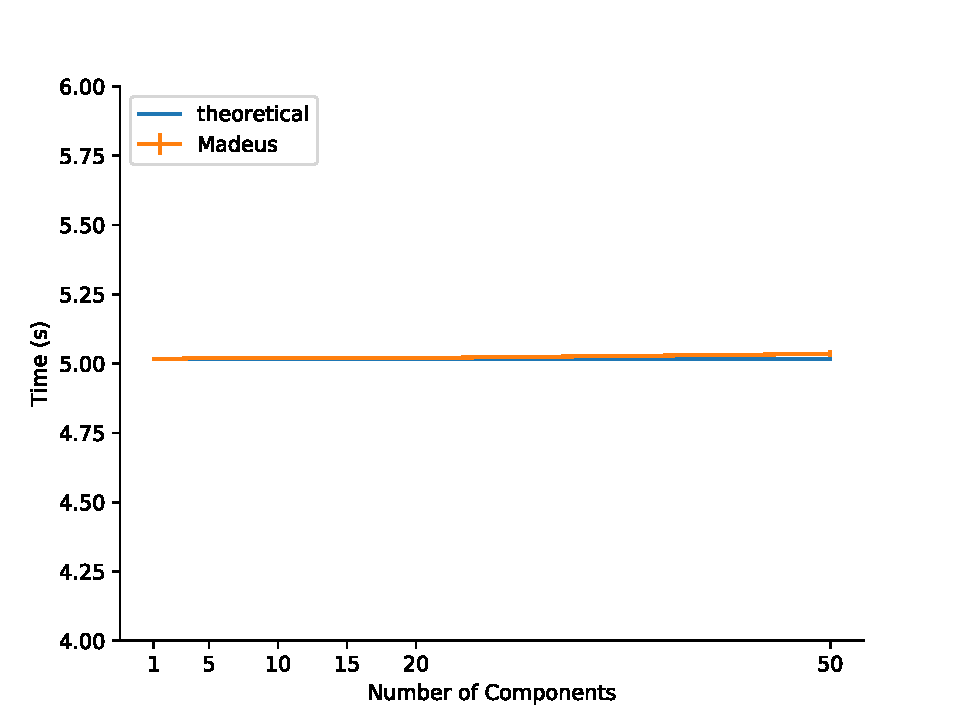
\includegraphics[width=0.5\textwidth]{./images/evaluations_par_component.pdf}
    \caption{Results of the parallel assembly benchmark with varying component number}
    \label{fig:parcompres}
  \end{center}
\end{figure}

For the results on the parallel assembly benchmark, we had to remove one outlier data point on the parallel assembly benchmark for component parallelism, as the first iteration of the assembly with just one component always had 4 seconds added to the time and we could not pinpoint the exact reason for that. As it did not occur for any of the other iterations, we did not take it into account on the curve drawing for our Figure~\ref{fig:parcompres}. In the results directory that can be found on our repository we have included the original times.json and the modified times.json files to keep the original results intact.

The ideal curve for the parallel assembly benchmark has been calculated with the \emph{sleep time} value on its own, if all the components are parallelized, they all start their transition at the same time and it should take only the \emph{sleep time} to be finished. In \emph{dryrun} our experimental benchmark is only very slightly above the ideal curve, which shows that Madeus does not add significant overhead to the process when there are more components. The \emph{ssh connection} curve allows us to see that there is steady increase of time, adding almost 3 seconds to the assembly deployment when reaching 40 parallel components. This show that the overhead added by the SSH connections is not null.

\begin{figure}[h]
  \begin{center} 
    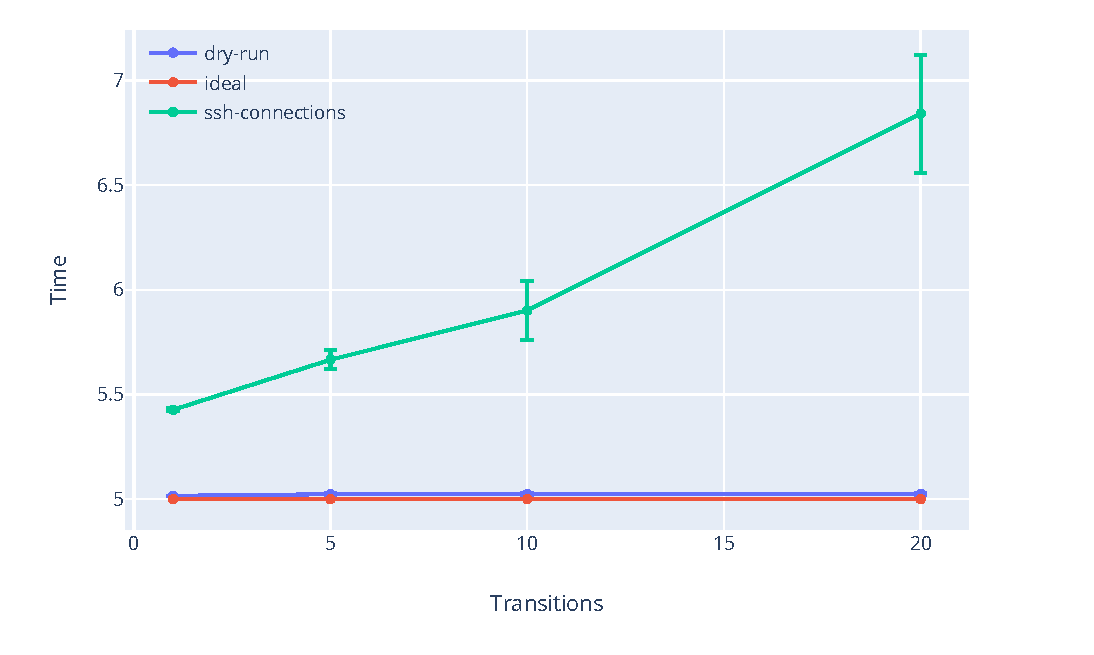
\includegraphics[width=0.5\textwidth]{./images/evaluations_par_transitions.pdf}
    \caption{Results of the parallel assembly benchmark with varying parallel transition number}
    \label{fig:partrans}
  \end{center}
\end{figure}

The results for the parallel assembly benchmark regarding parallel transition variation are illustrated on Figure~\ref{fig:partrans}. The calculation for the ideal curve on the parallel assembly benchmark when varying the number of parallel transitions has been done in the same manner as for the parallel component variation. In \emph{dryrun} the benchmark results follow the ideal curve closely as well, whereas the \emph{ssh connections} curve has an overhead that grows as the number of transitions increases.

These results allow us to point out that \emph{Madeus} does not by itself add a big overhead on the deployment. They also show the importance of ssh connection and their impact on the deployment time.

\subsection{Performance model precision}

\HC[All]{a voir}

